\documentclass[a4,danish]{article}

\usepackage{amssymb}
\usepackage{amsmath}
\usepackage{xcolor}
\usepackage{soul}
\usepackage{enumerate}

\newcommand{\Z}{\mathbb{Z}}
\newcommand{\Q}{\mathbb{Q}}
\newcommand{\R}{\mathbb{R}}
\newcommand{\N}{\mathbb{N}}
\newcommand{\C}{\mathbb{C}}
\renewcommand{\S}{\mathbb{S}}
\renewcommand{\P}{\text{P}}

\renewcommand{\phi}{\varphi}
\renewcommand{\epsilon}{\varepsilon}

\newcommand*\diff{\mathop{}\!\mathrm{d}}

\setlength{\parskip}{1em}
\setlength{\parindent}{0em}

% Figures -- use this instead of full file path because of git.
\usepackage{graphicx}
\graphicspath{{../figures/}}

\title{The tangent space of closed curves in $\R^2$}
\author{Mads and Anders}
\date{\today}

\begin{document}
% \maketitle

\section*{The tangent space of closed curves in $\R^2$}
\label{sec:tangent-space-closed}


\paragraph{Constructing the space of closed curves.}
Intuitively, we want to consider the space of all (smooth) closed
curves in $\R^2$. This can be seen as the space of all submanifolds in
$\R^2$ which are diffeomorphic to the unit circle $\S^1$. If we let
$\text{Imm}(\S^1,\R^2)$ denote the space of all \textit{immersion}
from the inut circle into the plane, we can define the space we
want to consider as
\begin{equation}
  \label{eq:curves}
  B :=
  \left\{
    q(\S^1) \mid q \in \text{Imm}(\S^1,\R^2)
  \right\}.
\end{equation}
Here we simply think of $q(\S^1) \subset \R^2$ as a subspace and forget
about the actual map $q$. (Keeping this mapping in mind we could
define the space in another way; but this is not so important right
now.)

\paragraph{The tangent space of B.}
For ordinary finite dimensional manifolds $B$, Lee defines the tangent
space at a point $p \in B$ through the notation of
\textit{derivations}; this is a rather abstract construction, but is
nice to work with. Using this, one can define the notion of a
tanget vector to a path in $B$ passing through the point $p$. Then,
one can define an equivalence relation on the space of such paths and
obtain an equivalent definition of the tanget space, which is more
intuitive. One can also work the other way around and start by
defining the notion of tanget vector to paths in $B$ (as is done on
Wiki). We briefly do that here:

For a neighbourhood $U \subset B$ containing $p$ we have a smooth coordinate
chart $\phi\colon U \rightarrow \R^n$. For a path $\gamma \colon
[-\epsilon,\epsilon] \rightarrow B$ with $\phi(0) = p$, it makes perfect sense to consider
differentiability of the map $\phi \circ \gamma \colon
[0,1]\rightarrow \R^n$. Now, the relation
\begin{equation*}
  \gamma_1 \sim \gamma_2 \iff
  (\phi \circ \gamma_1)'(0) = (\phi \circ \gamma_2)'(0),
\end{equation*}
defines an equivalence relation on the collection of all such paths
$\gamma$. An equivalence class of such paths, denoted by $[\gamma'_p]$ (or simply
$\gamma'_p$), is called a \textit{tangent vector}
at the point $p$. The collection of all tanget vectors make up the
tanget space $T_pB$ at $p$.

Returning to $B$ being as defined in (\ref{eq:curves}), we now
want to determine what the tangent spaces look like at a point $q \in B$ by
following the construction above (taking for
granted that $B$ actually is a (Fr\'echet) manifold, and
that the following definitions/constructions make sense). Firstly, a
path in $B$ is now a map $\gamma\colon [-\epsilon,\epsilon] \rightarrow B$ such that
$\gamma(t)$ is a curve $q_t \in B$ for all $t \in
[-\epsilon,\epsilon]$, with $\gamma(0) =q$. For each of the $q_t$ we
can think of them as parametrized by $x \mapsto q_t(x)$, $x \in
\S^1$. Then, if the curve $\gamma$ is such that for each fixed
$x \in \S^1 $ the map $t \mapsto q_{t}(x) \in \R^2$ is differentiable,
we can define $\gamma'_q$ as the mapping
\begin{equation*}
  \gamma'_q := x \mapsto \frac{\partial }{\partial t} \bigg\vert_{t=0}q_t(x).
\end{equation*}
Thus each $\gamma'_q$ is a mapping from the unit circle into $\R^2$,
which mean that we can think of a tangent vector to a curve $q \in B$
as a vector field on $\S^1$ (though of as $\subset \R^2$).


\paragraph{Question / considerations / imprecisions.}
Above we made an intuitively reasonable construction, but ignored some
of technicalities, which we list here.
\begin{itemize}
\item Equivalence classes: We should define the tangent vectors as
  equivalence classes of path in $B$; this should all determine a
  unique vector field.
\item The manifold structure of $B$: We simply used the intuitive idea
  to differentiate in ``time'' for each fixed point on a curve,
  $q_t(x)$. However, as we have not specified the chart for the
  manifold $B$, it is not obvious that this construction corresponds
  to the one made in the finite dimensional case. Technically we
  would need a chart $\phi \colon U \rightarrow F$, with $F$ some
  Fr\'echet space and then show some sort of Fr\'echet-differentiability of the
  composite function $\phi \circ \gamma$.
\item We mentioned that in the finite dimensional case the two
  definitions (through derivates and tangents to curves, respectively)
  are equivalent. It is not obvious that this also hold in the
  infinite dimensional case.
\item At the beginning we eliminated the knowledge of the
  parametrization of a curve $q \in B$ to make the definition of $B$
  simpler. However, we actually use a parametrization later, and thus
  we should make sure that reparametrizations does not matter for the
  construction of the tangent space. (It does not, as it would just
  move the vector field around $\S^1$ according to the
  reparametrization.)
\item Are there any smoothness assumptions (or something) about vector
  field we need to validate? For example, just the fact that the map
  $t \mapsto q_t(x)$ behaves nice does of course \textit{not} imply
  that also the derived vector field $\gamma'_q$ behaves nicely in
  $x$ -- which is what we would need to get a smooth vector field
  (?).
\item Is it correctly formulated that we need to think of $\S^1
  \subset \R^2$ to make sense of a vector field on the circle?
\end{itemize}


% \section*{Test section}
% \label{sec:test-section}

% \begin{center}
%   \begin{tikzpicture}
%     \begin{axis}[axis lines=none, axis equal,
%       width=0.9\textwidth,
%       xmin=-3,xmax=10,
%       ymin=-3,ymax=3,
%       % grid=both,
%       ]
%       \addplot [domain=0:360,samples=100]({2*cos(x)},{2*sin(x)});
%       \addplot[domain=0:360,samples=200]({7 +
%         (1-cos(x*2)/2)*1.8*sin(x)},{(1-sin(x*4)/2)*1.8*cos(x)});
%       \node[anchor=west] (source) at (axis cs:1.0,2.5){}; \node
%       (destination) at (axis cs:5.5,2.5){}; \draw[->](source) to
%       [out=40,in=140] (destination);
%     \end{axis}
%   \end{tikzpicture}
% \end{center}

% \begin{center}
%   \begin{tikzpicture}
%     \begin{axis}[axis lines=none, axis equal,
%       width=1\textwidth,
%       xmin=4,xmax=10,
%       ymin=-4,ymax=4,
%       ]
%       \addplot[domain=0:360,samples=200]({7 +
%         (1-cos(x*2)/2)*1.8*sin(x)},{(1-sin(x*4)/2)*1.8*cos(x)});

%       \addplot[domain=0:360,samples=200]({7 +
%         (1-0*cos(x*2)/2)*1.8*sin(x)},{1.2*(1-sin(x*4)/2)*1.8*cos(x)});

%       \foreach \t in {1,...,4}
%       \addplot[gray, domain=0:360,samples=200]
%       ({7 + (1-(1-\t /5)*cos(x*2)/2)*1.8*sin(x)},
%       {(1 + \t /25)*(1-sin(x*4)/2)*1.8*cos(x)});

%       \foreach \q in {1,...,72}
%       \addplot[->, red, domain=0:2.5,samples=5]
%       ({7 + (1-(1-x /5)*cos(\q *5*2)/2)*1.8*sin(\q *5)},
%       {(1 + x /25)*(1-sin(\q *5*4)/2)*1.8*cos(\q *5)});
%     \end{axis}
%   \end{tikzpicture}
% \end{center}


% \begin{center}
%   \begin{tikzpicture}
%     \begin{axis}[axis lines=none, axis equal,
%       width=1\textwidth,
%       xmin=4,xmax=10,
%       ymin=-4,ymax=4,
%       ]
%       \addplot[domain=0:360,samples=200]({7 +1 +
%         2*sin(x)},{2*cos(x)});

%       \foreach \q in {1,...,72}
%       \addplot[->, green, domain=0:2.5,samples=5]
%       ({7 + (1-(1-x /5)*sin(\q *5)*2},
%       {(1 + x /25)*2*cos(\q *5)});
%     \end{axis}
%   \end{tikzpicture}
% \end{center}

\section*{Test section 2}
\label{sec:test-section-2}

\begin{figure}
  \centerline{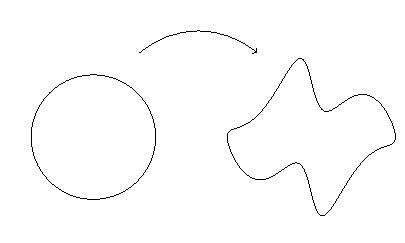
\includegraphics[width=0.7\linewidth]{circle_mapping.pdf}}
  % \caption[]{}
\end{figure}

\begin{figure}
  \centerline{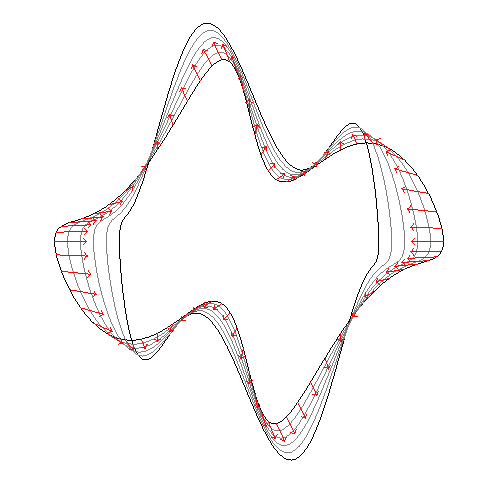
\includegraphics[width=0.7\linewidth]{path.pdf}}
  % \caption[]{}
\end{figure}

\begin{figure}
  \centerline{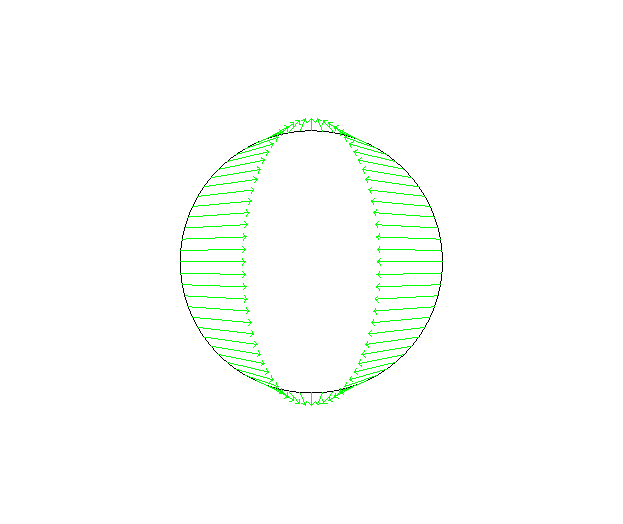
\includegraphics[width=0.7\linewidth]{circle_vectorfield.pdf}}
  % \caption[]{}
\end{figure}



\end{document}





